\begin{primeirapagina}
	\begin{abstract}
		\textbf{Resumo:}\\
Em 1978 Christopher T. Russell e Richard C. Elphic detectaram tubos de fluxo magnético na região de fronteira da magnetosfera terrestre por meio de dados observacionais obtidos pelos satélites ISEE-1 e -2, que foram denominados eventos de transferência de fluxo, ou simplesmente FTE (do inglês, flux transfer events). O vento solar, juntamente com o campo magnético interplanetário, oriundos do Sol, atingem a região de campo magnético terrestre, produzindo fenômenos como a reconexão magnética e os tubos de fluxo. Esse artigo apresenta uma introdução sobre a conexão Sol-Terra e o processo de reconexão magnética, e principalmente, os conceitos básicos sobre a geração e a formação dos tubos de fluxo magnético. Os modelos que descrevem o tipo de reconexão e as características dos tubos, como por exemplo Russell-Elphic, Lee-Fu e Southwood-Scholer, e as propriedades dos eventos FTE, são apresentados de forma clara e concisa. Por fim, o artigo trata de um exemplo de identificação dos tubos em simulação computacional, realizado nesse trabalho.\\
    \palavraschave{eventos de transferência de fluxo, física espacial, vento solar, reconexão magnética.}

	\end{abstract}

	\begin{abstract}
		\textbf{Abstract:}\\
In 1978 Christopher T. Russell and Richard C. Elphic detected magnetic flux tubes in magnetosphere boundary region through observational data obtained from the satellites ISEE-1 and -2, which were named flux transfer events (FTE). The solar wind together with the interplanetary magnetic field, both originated in the Sun, reach the earth magnetic field region, producing the magnetic reconnection and the flux tubes phenomena. This paper presents an introduction on the Sun-Earth connection and the magnetic reconnection process, and mainly the basic concepts on the tubes generation and formation. Themodelswhichdescribethetypeofreconnectionandthetubessignatures,forexample,Russell-Elphic, Lee-Fu, Southwood-Scholer, and the FTE event characteristics, are presented in a clear and concise way. Finally, this paper brings an example of the tubes identification in computing simulation, performed in this work.\\ 
	\keywords{flux transfer events, space physics, solar wind, magnetic reconnection.}
	
	\end{abstract}
\end{primeirapagina}

\saythanks

\normalsize
\baselineskip=12pt % Espaço de linha para a primeira pagina deve ser inicializado sempre q se use multicols


\section{A interação vento solar - magnetosfera terrestre}

O estudo da interação Sol-Terra tem se tornado cada vez mais necessário na sociedade, devido à crescente utilização de tecnologias espaciais e terrestres. Estes, por sua vez, são diretamente afetados pelo clima espacial, o qual refere-se às condições dinâmicas do ambiente espacial entre o Sol e a Terra, e também ao longo do sistema solar, que podem afetar as tecnologiais espaciais e terrestres.  \cite{gombosi2004,russell2001,oliveira2016,nstc2015}.

O Sol é a estrela do nosso sistema planetário e de grande importância para a humanidade, sendo composto por gases como hidrogênio e hélio. Essa estrela gera energia e radiação eletromagnética em diversos comprimentos de onda, por meio de reações termonucleares que ocorrem em seu núcleo. Além de luz e energia, o Sol é a origem do vento solar, que é um fluxo constante de partículas que permeia o meio interplanetário. Essas partículas são conhecidas como plasma, que é um gás, em sua maioria constituído por núcleos de hidrogênios e elétrons, altamente ionizado, macroscopicamente neutro e que possui comportamento coletivo \cite{baumjohann1996,bittencourt}. Esse comportamento coletivo ocorre devido às forças coulombianas de longo alcance presentes no plasma. O vento solar é resultado da diferença de pressão existente entre a coroa solar, a camada mais externa da atmosfera solar, e o espaço interplanetário. O plasma vence a força gravitacional do Sol e se expande pelo meio interplanetário. O campo magnético do Sol também se estende pelo meio interplanetário, sendo denominado campo magnético interplanetário ou IMF (do inglês, {/emph interplanetary magnetic field}) \cite{costa2011, kivelson1995}. 

O Sol apresenta ciclos de atividade solar com o período de aproximadamente 11 anos \cite{kivelson1995, costa2011}. Quando a atividade solar atinge seu máximo, a probabilidade de ocorrência de explosões solares aumenta. Essas condições pertubam o vento solar. Em condições ``calmas'', ou seja, durante baixa atividade solar, o vento solar apresenta as seguintes propriedades físicas na região da órbita da Terra (1 AU\footnote{AU é a sigla em inglês de \textit{Astronomical Unit}, referente à distância entre o Sol e a Terra que é de aproximadamente 150 milhões de quilômetros.}): velocidade de aproximadamente 400 $km/s$, densidade de aproximadamente 5 partículas$/cm^3$ e magnitude do campo magnético de cerca de 5 $nT$. Esse vento solar lento, é originado em regiões próximas ao equador do Sol. Por outro lado, o vento solar originado de buracos coronais no Sol, pode ser classificado como rápido, pois a sua velocidade atinge valores por volta de 800 km/s. Os buracos coronais são regiões mais frias e menos densas da coroa solar predominantemente localizadas em altas latitudes e formadas por linhas de campo magnético ``abertas''\footnote{Não existem literalmente linhas de campo magnético abertas devido à inexistência de monopolos magnéticos. Porém, esse termo é frequentemente usado para se referir a linhas de campo que se fecham a uma distância muito grande em relação ao Sol.} \cite{russell2001}.

O vento solar, juntamente com o campo magnético interplanetário, propaga-se pelo meio interplanetário e atinge o campo magnético terrestre, deformando-o. A magnetosfera é a região no espaço onde o campo magnético terrestre rege os processos físicos existentes. O campo magnético terrestre é gerado principalmente por correntes que circulam no interior do planeta e uma contribuição pequena é dada por sistemas de correntes atmosféricas e magnetosféricas.  

A Figura \ref{magnetosfera} apresenta as regiões mais importantes que compõem a magnetosfera terrestre \cite{russell2001,sibeck2014,ezequiel2006}. O lado diurno, que é a região voltada para o Sol no lado esquerdo da Figura \ref{magnetosfera}, estende-se, tipicamente, por 10 raios terrestres\footnote{1 raio terrestre (Re) é aproximadamente 6370 km.} em condições de vento solar calmo. As regiões observadas no lado diurno são principalmente: a frente de choque, que é a região onde as partículas são desaceleradas, funcionando como uma espécie de ``barreira'', e está representada por uma linha tracejada; a bainha magnética, que é uma região de forte turbulência entre a frente de choque e a magnetosfera; a magnetopausa, que é a região mais externa da magnetosfera, apresentando uma intensa densidade de corrente; e as cúspides polares, que são regiões nos pólos magnéticos onde a configuração das linhas de campo magnético terrestre facilitam a entrada de partículas na atmosfera terrestre.

O lado noturno (lado direito da Figura \ref{magnetosfera}), é conhecido como cauda magnetosférica ou magnetocauda, devido ao formato alongado provocado pelo arraste do vento solar. A magnetocauda pode chegar a distâncias superiores a 200 raios terrestres, sendo considerado um grande reservatório de energia e plasma \cite{russell2001,sibeck2014,ezequiel2006}.

\begin{figure}
	\begin{center}
		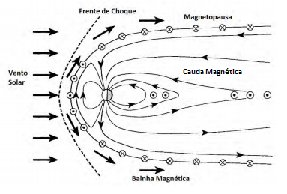
\includegraphics[scale=0.8]{magnetosfera.jpg}
		\caption[Fig]{Representação simplificada da magnetosfera terrestre que é formada a partir da interação do vento solar com o campo magnético terrestre. O lado diurno da magnetosfera corresponde ao lado esquerdo da imagem, direção na qual está situado o Sol, enquanto o lado noturno é a região da cauda, situada no lado direito. Fonte: Adaptado da Ref. \cite{elphic1979}}
		\label{magnetosfera}
	\end{center}
\end{figure}

Nos planetas que possuem campo magnético como a Terra, as magnetosferas funcionam como escudos protetores às partículas ionizadas oriundas do Sol. Entretanto, um fenômeno conhecido como reconexão magnética gera ``aberturas'' na magnetosfera e permite que as partículas adentrem o ambiente magnetosférico. Essa injeção de partículas gera perturbações no campo magnético terrestre. Um exemplo de um fenômeno bastante conhecido são as Auroras \cite{da2015,costa2011,souza2016,kivelson1995,baumjohann1996}, caracterizadas por emissões, em vários comprimentos de onda, geradas pela colisão entre as partículas oriundas do vento solar e da atmosfera terrestre.  


%%%%%%%%%%%%%%%%%%%%%%%%%%%%%%%%%%%%%%%%%%%%%%%%%%%%%%%%%%%%%%%%%%%%%%%%%%%%%%%%%%%%%%%%%%%%%%%%%%%%%%%%%%%%%%%%%%%%%%%%%%%%%%%%%%%
\section{Conceitos gerais sobre a reconexão magnética}

Em um plasma altamente condutor como o vento solar, o campo magnético se move junto com o plasma ao invés de difundir-se nele, como se estivessem ``congelados" entre si \cite{souza2016,costa2011}. O mecanismo de reconexão magnética está diretamente relacionado à condição de ``quebra do congelamento" do campo magnético, que corresponde à ocorrência do processo de difusão do campo magnético através do plasma. 

A reconexão magnética pode ser definida como a reestruturação topológica dos campos magnéticos causada pela mudança da conectividade das linhas de campo \cite{baumjohann1996}. No contexto da interação vento solar-magnetosfera, a reconexão ocorre geralmente quando as linhas de campo magnético terrestre e do meio interplanetário são antiparalelas. Esse mecanismo permite a passagem do plasma do vento solar para a magnetosfera através da magnetopausa terrestre. Ao longo de todo o processo de reconexão magnética, onde ocorre a fusão das linhas dos campos, o fluxo e a topologia dos campos se modificam, assim como ocorrem variações na velocidade das partículas e pressão do plasma.   

Para entender como ocorre a reestruturação topológica das linhas de campo na reconexão, considere duas linhas de campo magnético com sentidos aproximadamente antiparalelos sob o efeito de ``congelamento'', como mostrado na Figura \ref{reconexao}. As linhas de campo iniciam o processo de aproximação em um determinado ponto, como pode ser observado no Painel 1. Quando as linhas estão muito próximas, como no Painel 2, os campos não estão mais ``congelados'' ao plasma, permitindo a difusão. As linhas dos  dois campos diferentes se rearranjam, resultando na configuração de campo do Painel 3. As novas linhas de campo disparam em uma direção perpendicular à direção pela qual as linhas se aproximaram no início do processo e em sentidos opostos. 

O rompimento e o reagrupamento das linhas de campo magnético vistos na Figura \ref{reconexao} fazem parte do fenômeno de reconexão magnética. Como as linhas, após serem reconectadas, se propagam em sentidos opostos, o vetor velocidade das partículas envolvidas no processo é um importante parâmetro para identificar o fenômeno de reconexão na magnetopausa terrestre.

\begin{figure} [ht]
	\begin{center}
		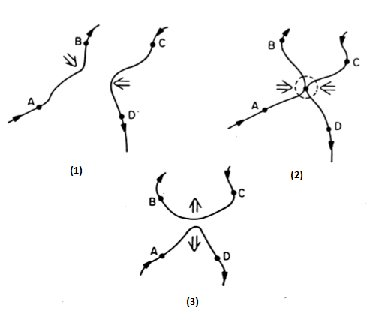
\includegraphics[scale=0.65]{reconexao.jpg}
		\caption{Fases do mecanismo de reconexão magnética: (1) a aproximação das linhas de campos magnéticos distintos, (2) o rompimento de ambas em um determinado ponto e (3) o reagrupamento das linhas produzindo o surgimento de duas novas linhas reconectadas que se propagam na direção perpendicular à direção de fluxo de plasma em (1). Fonte: Ref. \cite{lakhina1992}.}
		\label{reconexao}
	\end{center}
\end{figure} 

Existem diversos modelos teóricos que tentam explicar o processo físico da reconexão magnética. Eles são baseados principalmente em análises de dados e simulações numéricas. Dentre os mais importantes modelos estão o de Sweet-Parker e o de Petschek.

O modelo de Sweet-Parker é conhecido por explicar o processo de reconexão lento. O modelo é baseado na conservação de massa, momento, energia e fluxo magnético para plasmas ideais entrando e saindo da região de difusão. Essa região se estende ao longo da fronteira entre dois campos magnéticos distintos e antiparalelos, como pode ser observado na Figura \ref{sweetparker}. As dimensões da região de difusão são formadas pelo comprimento 2\textit{L} e pela espessura 2\textit{l}. A reconexão magnética é mantida pelo balanço entre o fluxo de plasma que entra na região de difusão de largura 2\textit{l} e o fluxo de plasma que sai ao longo da lâmina de corrente de comprimento 2\textit{L}\cite{treumann}.

\begin{figure}
	\begin{center}
		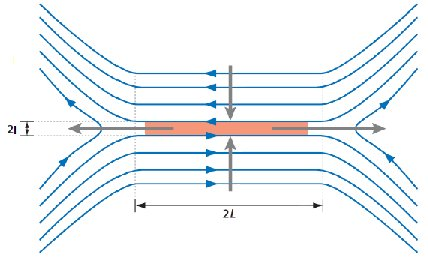
\includegraphics[scale=0.55]{sweetparker.jpg}
		\caption{Esquema do mecanismo de reconexão magnética no modelo de Sweet-Parker. Fonte: Adaptado da Ref. \cite{zweibel2009}. }
		\label{sweetparker}
	\end{center}
\end{figure} 

Entretanto, o modelo de Sweet-Parker requer uma extensa camada de corrente e por isso o processo de reconexão é muito lento. Petschek apresentou em 1964 um novo mecanismo que tenta explicar como ocorre o processo de reconexão rápida. Nesse modelo, representado na Figura \ref{petschek}, Petschek propôs uma região de difusão bem menor que a proposta por Sweet-Parker, limitada por um pequeno comprimento \textit{l} na fronteira entre os campos magnéticos de sentidos opostos (ao longo do eixo \textit{z}). Quando a região de difusão, que possui condutividade finita, é restrita a uma menor região do espaço o processo de reconexão se torna mais rápido, resolvendo o problema do modelo de Sweet-Parker. 

Além disso, foram introduzidas quatro frentes de choque conectadas à região de difusão, localizadas nas linhas diagonais tracejadas da Figura \ref{petschek}. Essas ondas de choque mudam a direção do campo magnético causando uma rotação de 90 graus. Esse campo que sofreu rotação é o campo reconectado que deixa a região de difusão e é conduzido pela força magnética \cite{treumann}. 

\begin{figure}
	\begin{center}
		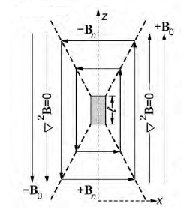
\includegraphics[scale=0.9]{petschek.jpg}
		\caption{Esquema do mecanismo de reconexão magnética no modelo de Petschek. Fonte: Adaptado da Ref. \cite{treumann}. }
		\label{petschek}
	\end{center}
\end{figure} 


%%%%%%%%%%%%%%%%%%%%%%%%%%%%%%%%%%%%%%%%%%%%%%%%%%%%%%%%%%
\section{Os tubos de fluxo magnético}
\label{FTE}

O processo de reconexão magnética é caracterizado por variações temporais e espaciais \cite{gonzalez1974,elphic1978}. As variações temporais podem ser lentas (ou estacionárias), com a duração da ordem de horas, ou rápidas (ou transientes), referindo-se a duração de alguns minutos. Em termos de variações espaciais, o processo de reconexão pode ocorrer em extensas regiões da magnetosfera, da ordem de alguns raios terrestres, sendo denominado global. Por outro lado, o processo pode ser localizado, ocorrendo em uma região pequena de aproximadamente 1 raio terrestre, ou até menor.   

As características espaciais e temporais do mecanismo formam os modos de reconexão magnética. Os modos mais conhecidos, encontrados em dados observacionais, são a reconexão global/estacionária \cite{gonzalez1974} e a localizada/transiente \cite{elphic1978}. Outras combinações entre esses modos de reconexão são possíveis.

A região ao longo do qual ocorre o processo de reconexão é caracterizada por campo magnético nulo. Essa região pode ser entendida como um prolongamento de vários pontos de reconexão e é denominada linha-X ou linha de reconexão\cite{gonzalez1974}. A orientação da linha de reconexão é influenciada pela direção do campo magnético interplanetário. Os modelos sugerem a existência de uma única linha-X \cite{southwood1988,scholer1988} ou de múltiplas linhas \cite{lee1985}.

A reconexão magnética transiente forma estruturas conhecidas como tubos de fluxo magnético. Os tubos que satisfazem os critérios impostos por Russel e Elphic \cite{elphic1978} são denominados eventos de transferência de fluxo ou FTE. Esses eventos ocorrem na magnetopausa terrestre e foram primeiramente identificados por Russel e Elphic \cite{elphic1978} e Haerendell et al. \cite{haerendel1978}, independentemente, por meio de alterações nos dados do campo magnético obtidos pelos satélites.


\subsection{Modelos de formação e geração dos tubos de fluxo}
\label{modeloRussel}

Russell e Elphic, em 1978, publicaram o artigo \cite{elphic1978} que trazia os primeiros resultados obtidos pelos magnetômetros da missão ISEE-1 e -2 (\textit{International Sun-Earth Explorer}). Esses resultados mostravam as medições das sondas, que estavam separadas por cerca de 360 quilômetros, em quatro diferentes passagens ao longo da magnetopausa, que é o local de ocorrência dos eventos.

Em sua análise, Russell e Elphic optaram por um sistema de coordenadas especial, baseado na direção normal à magnetopausa. Esse sistema é composto por uma componente normal à magnetopausa local, definido como \textbf{n}, uma componente \textbf{l}, projetada no plano perpendicular à direção normal e apresentando uma direção aproximadamente norte-sul, e uma componente \textbf{m} definida como $\textbf{n}\times \textbf{l}$, que completa o conjunto ortogonal. O propósito na escolha desse sistema de coordenadas local, ao invés de um global, foi facilitar a interpretação dos dados e a detecção dos FTEs. É extremamente importante ressaltar a importância da definição desse sistema de coordenadas normal à magnetopausa, já que é um dos motivos atribuídos ao sucesso da identificação dos eventos de transferência de fluxo.

Existem algumas técnicas e modelos para obter a posição da magnetopausa e a sua direção normal. A magnetopausa pode variar sua posição em relação a Terra, dependendo da atividade solar. Um dos modelos utilizados por Russell e Elphic para construir esse sistema de coordenadas foi considerar uma geometria cônica com excentricidade 0,4 com foco na Terra \cite{elphic1978}. Outro modelo muito utilizado é o de mínima variância, que pode ser encontrado com mais detalhes nas referências \cite{sonnerup1967} e \cite{siscoe1968}. 

Os tubos de fluxo magnético denominados FTEs são identificados por variações no campo magnético nas direções \textbf{l, m, n} e na magnitude total (módulo). A Figura \ref{bipolar} mostra os resultados obtidos pelos magnetômetros ISEE-1 e ISEE-2 para um dos cruzamentos que ocorreu no dia 8 de novembro de 1977, onde o campo magnético interplanetário tinha orientação sul. Os eventos FTEs estão identificados entre as linhas pontilhadas, iniciando nos instantes\footnote{A notação utilizada ao longo deste artigo será sempre da forma horas:minutos:segundos.} 02:12:00, 02:34:00 e 02:54:00. A característica principal desse evento é a natureza bipolar da componente $B_n$, em que atinge picos positivos (ou negativos) e em seguida descresce (cresce) para picos negativos (ou positivos). As outras componentes $B_l$, $B_m$, e a intensidade total $|B|$ são intensificadas.   

\begin{figure}
	\begin{center}
		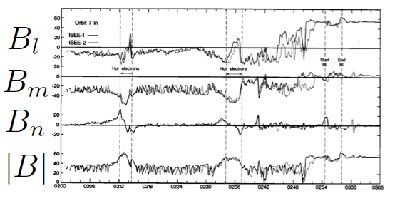
\includegraphics[scale=0.9,angle=90]{bipolar.jpg}
		\caption{Identificação dos FTEs encontrados por Russell e Elphic (1978) através de medidas de campo magnético realizadas pelos satélites ISEE-1 e -2 no cruzamento da magnetopausa em 8 de novembro de 1977. As regiões delimitadas pelas linhas verticais pontilhadas indicam a ocorrência de FTEs. Fonte: Adaptado da Ref. \cite{elphic1978}.  }
		\label{bipolar}
	\end{center}
\end{figure}

Russell e Elphic tentaram compreender o comportamento peculiar das variações do campo magnético identificadas na Figura \ref{bipolar}, que foram detectadas simultaneamente nas duas sondas ISEE-1 e -2. A coerência dos sinais demonstra que as sondas detectaram o mesmo evento, que se propagou ao longo da magnetopausa, passando pelos satélites. A estrutura do FTE foi caracterizada como um tubo de fluxo magnético na forma de um ``cotovelo'' (em inglês, \textit{elbow shaped}), como pode ser observado na Figura \ref{russel}(a). 

A formação do tubo de fluxo magnético foi atribuída como uma consequência do processo de reconexão magnética transiente e localizada \cite{elphic1978}.  O campo magnético interplanetário, identificado pelas linhas inclinadas na Figura \ref{russel}(a), é reconectado com o campo magnético terrestre, que correspondem às linhas verticais. Essa reconfiguração dos campos magnéticos forma um tubo de fluxo magnético, que pode se deslocar ao longo da magnetopausa devido às forças de tensão magnética e de arraste provocado pela propagação do vento solar.

\begin{figure}
	\begin{center}
		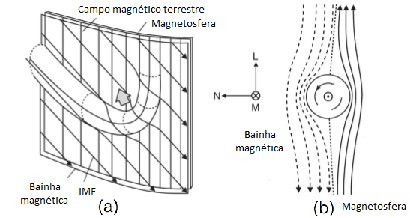
\includegraphics[scale=0.6]{russel.jpg}
		\caption{ Modelo de Russell-Elphic para os FTEs. (a) Tubo de fluxo magnético na forma de um ``cotovelo''. (b) Corte na seção transversal do tubo de fluxo, mostrando a rotação do campo magnético responsável pela assinatura bipolar da componente normal do campo. Fonte: Adaptado da Ref. \cite{elphic1978} e \cite{paschmann1982}. }
		\label{russel}
	\end{center}
\end{figure}


Um campo magnético na forma helicoidal foi identificado no interior do FTE, como pode ser observado na Figura \ref{russel}(b), que mostra um corte transversal do tubo de fluxo magnético. Quando o satélite passa através do tubo, o instrumento detecta a mudança de sentido da componente normal do campo magnético, indo de valores positivos para negativos ou vice-versa, correspondendo a característica de bipolaridade de \textbf{$B_n$}. 

A teoria proposta por Russell e Elphic \cite{elphic1978} é apenas um dos diversos modelos existentes que tentam explicar a formação dos eventos de transferência de fluxo. Todavia, existem outros dois modelos que são bastante conhecidos e difundidos na literatura, Lee-Fu \cite{lee1985} e Southwood-Scholer \cite{southwood1988,scholer1988}.

O trabalho de Lee-Fu explica a formação de tubos de fluxo magnético como resultado de múltiplas linhas de reconexão \cite{lee1985}. A Figura \ref{leeefu} retrata esse modelo, onde podem ser observadas três linhas-X, que possuem uma longa extensão azimutal ao longo da magnetopausa e são indicadas por linhas tracejadas. Como resultado da reconexão magnética, dois tubos de fluxo magnético são formados, compostos por campo magnético helicoidal, como mostra a Figura \ref{leeefu}. Esses tubos deslocam-se em direção aos pólos magnéticos devido à tensão magnética. Nesse modelo de múltiplas linhas de reconexão, o número de tubos formados é igual ao número de linhas-X menos um. No caso da Figura \ref{leeefu}, são três linhas-X e dois tubos de fluxo magnético formados. 

\begin{figure}
	\begin{center}
		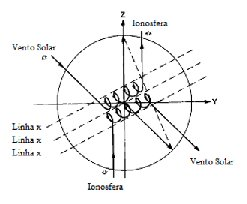
\includegraphics[scale=0.8]{leeefu.jpg}
		\caption{ Modelo de FTE originado por múltiplas linhas-X, proposto por Lee e Fu em 1985. Fonte: Adaptado da Ref. \cite{lee1985}. }
		\label{leeefu}
	\end{center}
\end{figure}

Southwood e Scholer independentemente propuseram em 1988 um modelo para a formação de FTEs baseado em uma única linha de reconexão \cite{southwood1988,scholer1988}. Como resultado, ocorre a formação de dois tubos com longa extensão azimutal. Esses tubos são formados pelo acúmulo de linhas de campo magnético dando origem a protuberâncias, como pode ser observado na parte superior da Figura \ref{southwood2}. A propagação dos tubos pode ser observada na parte inferior da Figura \ref{southwood2}. Nessa situação, o comportamento bipolar da componente normal do campo magnético aparece devido à propagação dos tubos. 

\begin{figure}
	\begin{center}
		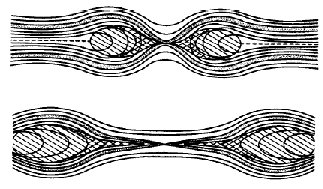
\includegraphics[scale=0.7]{southwood2.jpg}
		\caption{Modelo de FTE originado por uma única linha-X, proposto por Southwood e Scholer em 1988. Fonte: Adaptado da Ref. \cite{southwood1988}. }
		\label{southwood2}
	\end{center}
\end{figure}

Além dos três principais modelos mencionados anteriormente, Russell-Elphic, Lee-Fu e Southwood-Scholer, que descrevem a geração dos FTEs e a forma dos tubos de fluxo, existem outros trabalhos recentes que obtiveram diferentes resultados. Um evento FTE formado por dois tubos de fluxo magnéticos interlaçados, como no esquema da Figura \ref{hesse}, foi observado em resultados de modelos de simulação computacional, modelos numéricos e até mesmo de dados observacionais \cite{hesse1990,lee1993,otto1995,louarn2004,cardoso2013}. A forma dos tubos de fluxo é similar àquela descrita pelo modelo de Russell-Elphic, entretanto, os dois tubos estão interligados. De acordo com \cite{cardoso2013}, o conjunto dos dois tubos se enquadra na descrição de um FTE definida por \cite{elphic1978}. O mecanismo de geração desse FTE foi atribuído a múltiplas linhas de reconexão, como no modelo de Lee-Fu \cite{cardoso2013}.

\begin{figure}
	\begin{center}
		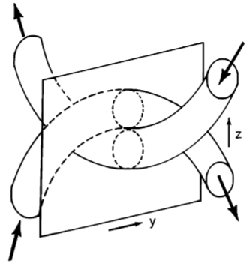
\includegraphics[scale=0.6]{hesse.jpg}
		\caption{Representação dos tubos de fluxo interlaçados. Fonte: Ref. \cite{hesse1990}. }
		\label{hesse}
	\end{center}
\end{figure}


\subsection{Características dos eventos FTEs}
\label{caracteristicas}

Como mencionado anteriormente, a principal característica dos FTEs, que pode ser identificada nos dados observacionais, é a variação bipolar da componente $B_{n}$ do 
campo magnético, geralmente centrada no máximo da intensidade total do campo. Os FTEs observados por Russell e Elphic em 1978 possuíam variação bipolar positiva/negativa 
($+/-$), sendo convencionados como FTEs padrão. Os trabalhos subsequentes reportaram observações de FTEs com a variação de $B_{n}$ com ``polaridade'' oposta ($-/+$),
denominados FTEs reversos \cite{Rijnbeeketal1982}. Percebeu-se então que o  sinal da variação bipolar é o resultado do movimento relativo entre a estrutura e o
satélite observador. 

Em uma primeira aproximação, o sinal da variação de $B_{n}$ pode indicar a posição da região de reconexão que originou o FTE. Para um FTE com polaridade padrão, a região 
de reconexão está ao sul do satélite observador como é mostrado nas Figuras \ref{fbn1}(a) e (b) \cite{paschmann1982}. Por outro lado, a observação de um FTE reverso 
indica que a região de reconexão está ao norte do satélite observador, como é mostrado nas Figuras \ref{fbn2}(a) e (b) \cite{paschmann1982}. 

As Figuras \ref{fbn1}(a) e \ref{fbn2}(a) mostram o corte transversal de um tubo de fluxo na magnetopausa, onde a posição da linha de reconexão é indicada por uma linha
tracejada, a seta verde mostra a direção e o sentido de propagação da estrutura, as setas vermelhas se referem à direção e ao sentido da componente normal do campo magnético,
o pentágono rosa representa a posição do satélite observador. A linha-X está na direção {/textbf m}. As Figuras \ref{fbn1}(b) e \ref{fbn2}(b) exibem a série temporal da intensidade do campo magnético $\left|B\right|$ e da componente $B_{n}$.

\begin{figure}
	\begin{center}
		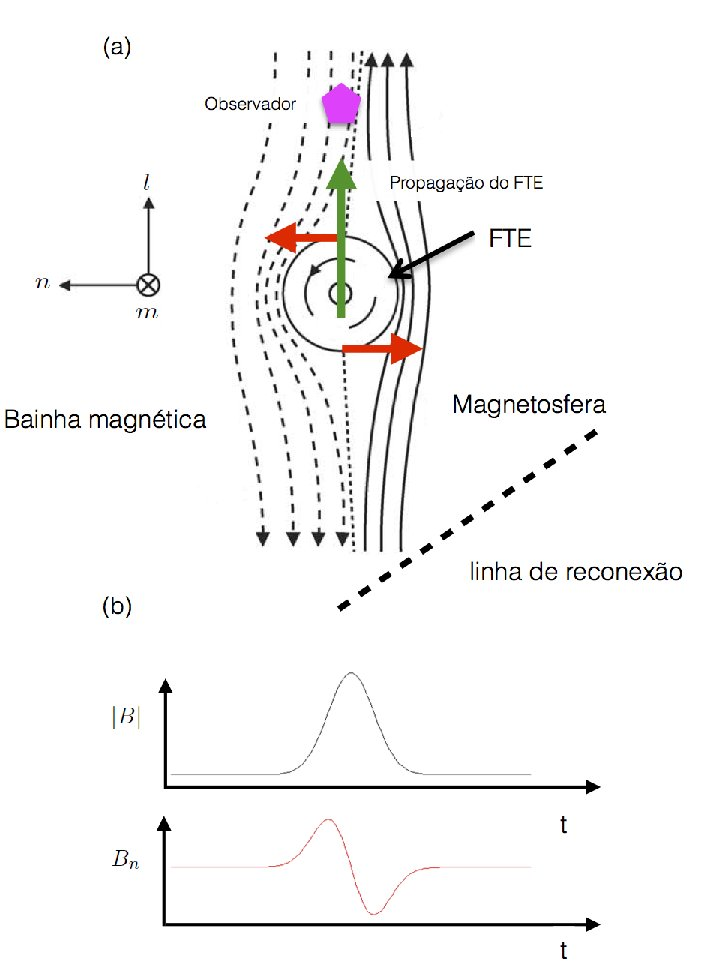
\includegraphics[scale=0.27]{fbn_fte_1.jpg}
		\caption{Características de um evento FTE: relação entre a variação bipolar de $B_{n}$ e o satélite observador com a região 
			de reconexão ao sul do satélite observador. Fonte: Adaptado da Ref. \cite{paschmann1982}.}
		\label{fbn1}
	\end{center}
\end{figure}

\begin{figure}
	\begin{center}
		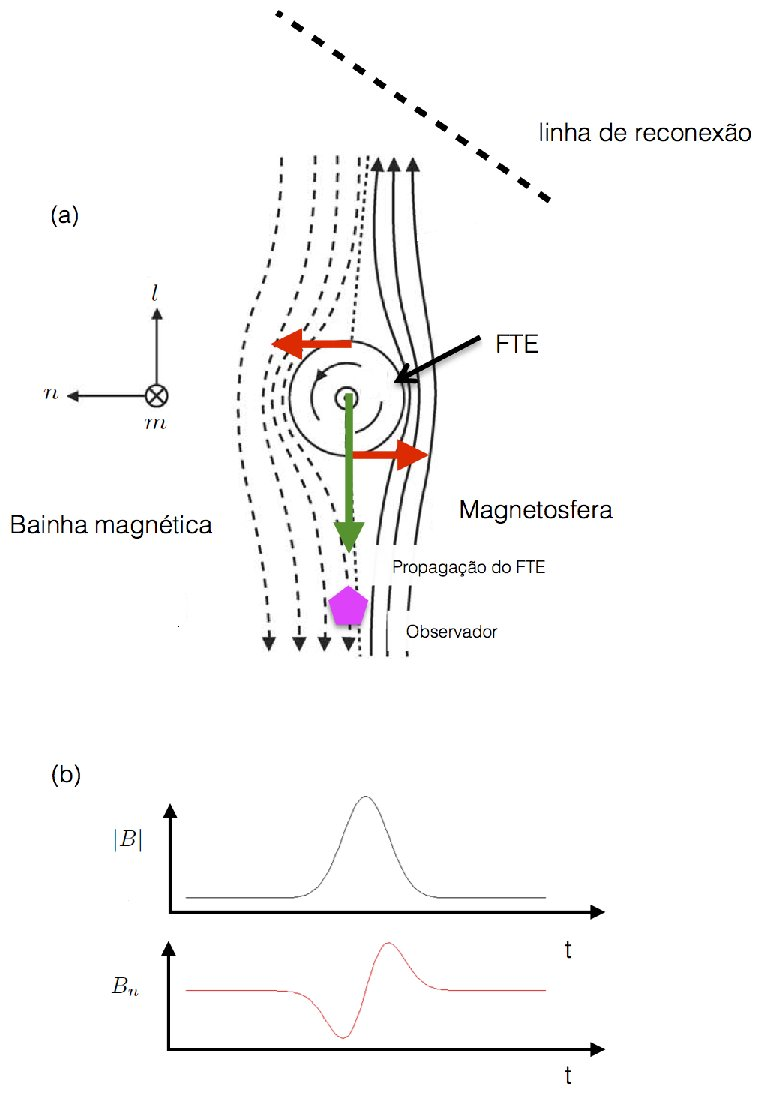
\includegraphics[scale=0.27]{fbn_fte_2.jpg}
		\caption{Características de um evento FTE: relação entre a variação bipolar de $B_{n}$ e o satélite observador com a região de reconexão ao norte do satélite observador. 
			Fonte: Adaptado da Ref. \cite{paschmann1982}.}
		\label{fbn2}
	\end{center}
\end{figure}

Na situação da Figura \ref{fbn1}(a), o FTE com polaridade padrão se origina na linha-X localizada na parte inferior do esquema. Durante o movimento do FTE, o satélite 
primeiramente detecta a componente $B_{n}$ positiva, indicada pela seta vermelha que aponta em direção à bainha magnética, e depois, a componente negativa, representada 
pela seta vermelha na direção da magnetosfera. A magnitude $\left|B\right|$ é intensificada e a componente $B_{n}$ é caracterizada pela variação bipolar positiva/negativa 
($+/-$) na Figura \ref{fbn1}(b). 

O FTE com polaridade reversa é gerado na linha-X localizada na parte superior da Figura \ref{fbn2}(a). O FTE se propaga ao longo da magnetopausa e o satélite mede a variação
bipolar negativa/positiva ($-/+$), indicada pelas setas vermelhas que apontam primeiramente em direção à magnetosfera e depois para a bainha magnética. A Figura \ref{fbn2}(b) mostra a intensificação da magnitude $\left|B\right|$ e a variação bipolar da componente $B_{n}$.

Com o aumento das missões espaciais priorizando a magnetosfera diurna da Terra, tornou-se possível a realização de diversos estudos sobre a ocorrência dos FTEs. Por meio da análise dos dados obtidos pelos satélites, observou-se que os FTEs com polaridade padrão tendem a ser detectados acima do equador magnético, no plano da eclíptica, enquanto que os FTEs com polaridade reversa são vistos abaixo do equador magnético. Esses resultados podem ser encontrados em \cite{BerchemandRussell1984}, \cite{Rijnbeeketal1984} e \cite{Russelletal1996}. 

Embora os FTEs possam ser observados ao longo de toda a magnetopausa, há uma maior probabilidade de sua ocorrência em médias latitudes magnéticas do que na região equatorial \cite{BerchemandRussell1984}. Entretanto, os modelos numéricos sugerem que as variações geradas pelos FTEs em seu ambiente aumentam à medida que se afastam da região equatorial \cite{SibeckandLin2010}, podendo ser mais facilmente detectadas em latitudes médias. A distribuição dos FTEs na magnetopausa é também influenciada pela direção do campo magnético interplanetário, uma vez que este último é o responsável pela orientação da linha-X \cite{Russelletal1985,Fearetal2009,Silveira2015}.

Diversos trabalhos descrevendo as características do comportamento do campo magnético e do plasma dentro e na vizinhança das estruturas magnéticas foram publicados ao longo dos anos. Os FTEs podem apresentar variações em parâmetros como temperatura, densidade e velocidade média do plasma \cite{Elphic1995,Paschmannetal1982}.  A coexistência de plasma da bainha magnética e da magnetosfera no interior dos tubos de fluxo, além de haver aceleração associada à componente norte-sul do fluxo de plasma, corroboraram com a hipótese da reconexão magnética ser o mecanismo gerador dos FTEs \cite{Paschmannetal1982}. 

Os FTEs ocorrem em intervalos de aproximadamente 8 minutos \cite{Rijnbeeketal1984}, ou seja, um novo FTE é gerado a cada 8 minutos quando o processo de reconexão favorece a formação do evento. As dimensões características de um FTE podem variar de 0,4 a 4 raios terrestres na direção normal à magnetopausa \cite{Owenetal2001} e podem ter mais de 10 raios terrestres na sua direção azimutal \cite{Fearetal2008}.

A monografia publicada em 1995 na \textit{American Geophysical Union} por Elphic \cite{Elphic1995} sugere uma classificação taxonômica para os FTEs. A Figura \ref{tipofte} mostra traços idealizados das características dos FTEs nas componentes do sistema de coordenadas normal à magnetopausa $B_{l}$, $B_{m}$ e $B_{n}$, intensidade do campo $|B|$, densidade de partículas $N$, módulo da velocidade do plasma $V$, temperatura média $T$ e fluxo de partículas energéticas $EP$. Cada coluna vertical do painel mostra as características dos tipos de FTE, A, B, C e D, em todos os parâmetros mencionados. 

As categorias A e B são ligeiramente semelhantes. Entretanto, a componente $B_m$ é mais evidente e a componente $B_n$, juntamente com $|B|$, são levemente intensificadas no evento FTE tipo B. A categoria C apresenta uma mudança de $B_{l}$ para norte e o campo magnético total $|B|$ tem valor mínimo nas bordas do tubo de fluxo. A categoria D representa a observação de um FTE no momento em que o satélite cruza a magnetopausa.

\begin{figure} [ht]
	\begin{center}
		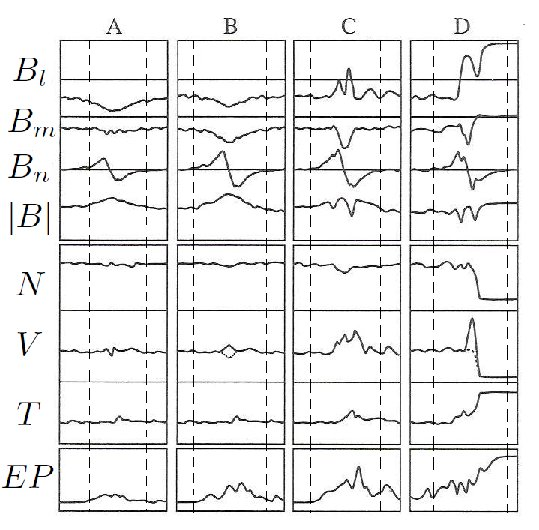
\includegraphics[scale=0.45]{tipofte.jpg}
		\caption{Perfis de assinaturas de quatro diferentes tipos de FTEs (A,B,C e D) em parâmetros observacionais: componentes do sistema de coordenadas normal à magnetopausa $B_{l}$, $B_{m}$ e $B_{n}$, intensidade do campo $|B|$, densidade de partículas $N$, módulo da velocidade do plasma $V$, temperatura média $T$ e fluxo de partículas energéticas $EP$. Fonte: Ref. \cite{Elphic1995}.}
		\label{tipofte}
	\end{center}
\end{figure}

As perturbações causadas pelos FTEs podem ser observadas nas proximidades da Terra, especificamente na ionosfera\footnote{Ionosfera é uma camada de plasma que envolve a Terra e forma a interface entre a atmosfera terrestre e o espaço. A altura da camada pode variar de algumas dezenas a centenas de quilômetros \cite{kelley}.} devido ao mapeamento do campo magnético equatorial para regiões polares. Tais perturbações podem ser detectadas através do fluxo de plasma observado por radares, câmeras \textit{all-sky} e fotômetros. Diversos estudos demonstram a ligação entre FTEs observados na magnetopausa e jatos de fluxo de plasma observados na ionosfera \cite{Fearetal2009,pinnock03,gary90}. Também foram observados eventos de expansão de aurora no lado diurno, próximo às bases das linhas de campo magnético da região observada na região equatorial \cite{Elphicetal1990,GlassmeierandStellMacher1996,Neudeggetal2000}. 


\section {Exemplo de identificação de tubos de fluxo magnético em simulação computacional}

Os primeiros FTEs foram identificados basicamente por meio de alterações do campo magnético \cite{elphic1978}. Entretanto, as regiões de reconexão, e consequentemente os tubos, também podem ser detectados por mudanças na velocidade. Como apresentado na Figura \ref{reconexao}, as linhas reconectadas de campo magnético disparam em uma direção perpendicular à direção pela qual as linhas se aproximaram no início do processo e em sentidos opostos. 

Em simulação computacional, é possível identificar os tubos de fluxo magnético utilizando-se dos parâmetros apropriados, como por exemplo, pressão, campo magnético e velocidade. Como essas estruturas magnéticas possuem extensas dimensões tridimensionais ao longo da magnetopausa, a análise dos resultados de simulação permite uma caracterização mais conveniente das formas e dos tamanhos dos tubos do que os dados pontuais obtidos por satélites. 

Analisaremos um caso de simulação computacional da interação entre o vento solar e a magnetosfera terrestre, onde os tubos de fluxo magnético são identificados. Nesse caso, o vento solar, antes de interagir com a magnetosfera, possui características de campo magnético e velocidade intensos e estacionários, em que as condições impostas como iniciais, são: as componentes\footnote{Coordenadas GSM ({/emph Geocentric Solar Magnetospheric}), onde {/emph x} está na linha que liga o Sol à Terra com sentido positivo apontando para o Sol, {/emph z} é a projeção do dipolo magnético terrestre na direção perpendicular a {/emph x}, apontando para sentido norte, e {/emph y} completa o sistema ortogonal.} $y$ e $z$ do campo magnético interplanetário possuem os valores de $+14$ $nT$ e $-14$ $nT$, a componente $x$ da velocidade do vento solar é $- 600 km/s$ e a densidade tem o valor de 5 partículas$/cm^3$ \cite{cardoso2013}.

Esse caso de simulação foi processado na {/emph Nasa Community Coordinated Modeling Center} (NASA CCMC) e o código computacional utilizado é denominado BATS-R-US ({/emph Block-Adaptative-Tree-Solarwind-Roe-Upwind-Scheme}) \cite{toth05,gombosi2004,powell99}. O modelo é baseado na teoria magnetohidrodinâmica (MHD), que considera o plasma como um fluido magnetizado \cite{bittencourt,baumjohann1996}.

No trabalho de Cardoso e colaboradores \cite{cardoso2013}, foram identificados tubos de fluxo magnético interlaçados no instante de tempo 00:23:00, no mesmo caso de simulação analisado nesse artigo. O tempo total de simulação é de 45 minutos, o que significa que a simulação do processo de interação entre o vento solar e a magnetosfera tem duração de 45 minutos. 

Nesse artigo, como exemplo para identificação de tubos de fluxo magnético, foi analisado o evento ocorrido no instante de tempo 00:30:00. Os parâmetros de pressão de plasma, campo magnético e velocidade são analisados de forma que o mecanismo de reconexão magnética e os tubos de fluxo possam ser identificados e caracterizados. 

A análise da pressão de plasma possibilita a detecção dos tubos de fluxo, embora não permita a caracterização da forma dos tubos de fluxo magnético. A Figura \ref{pressaotempo} apresenta a pressão de plasma no plano $x-z$ em $y= -0,5$ $Re$ no instante 00:31:30 (painel esquerdo) e 00:32:00 (painel direito). O Sol está localizado à direita e a Terra na origem do sistema de coordenadas em todos os gráficos apresentados nessa Seção. A protuberância na cor vermelha corresponde à intensificação da pressão no tubo que se origina na região ao sul do equador, entre $z= 0$ e $-1$ $Re$. O tubo se propaga ao longo da magnetopausa para o norte, conforme pode ser observado no painel direito. 

A topologia magnética mostra a conectividade das linhas de campo e é uma ferramenta essencial para a caracterização dos tubos de fluxo magnético. A Figura \ref{topologia} apresenta a topologia magnética para os instantes de tempo 00:31:00 (painel esquerdo) e 00:31:30 (painel direito) no plano $x-z$ em $y= 0$. As regiões são identificadas em cores: vermelha corresponde à região em que as linhas estão conectadas à Terra, azul identifica as linhas ligadas ao Sol, verde corresponde às linhas que são conectadas ao sul da Terra e ao Sol e amarela para as linhas conectadas ao norte da Terra e ao Sol. O local em que as quatro cores se encontram pode ser um provável local de reconexão \cite{cardoso2013,dorelli09,raeder06}. No instante 00:31:00, as pequenas regiões nas cores verde e amarela entre $z= - 0,3$ e $-0,9$ $Re$ localizadas na magnetopausa correspondem aos tubos de fluxo magnético produzidos pelo mecanismo de reconexão magnética. Para que a estrutura do tubo possa ser caracterizada em termos de dimensão e forma, é necessário que a topologia magnética seja analisada em vários planos. Como o tubo se propaga para o norte, conforme observado na Figura \ref{pressaotempo}, a topologia magnética se torna mais complexa, como mostra o painel direito da Figura \ref{topologia}.

\begin{figure}
	\begin{center}
		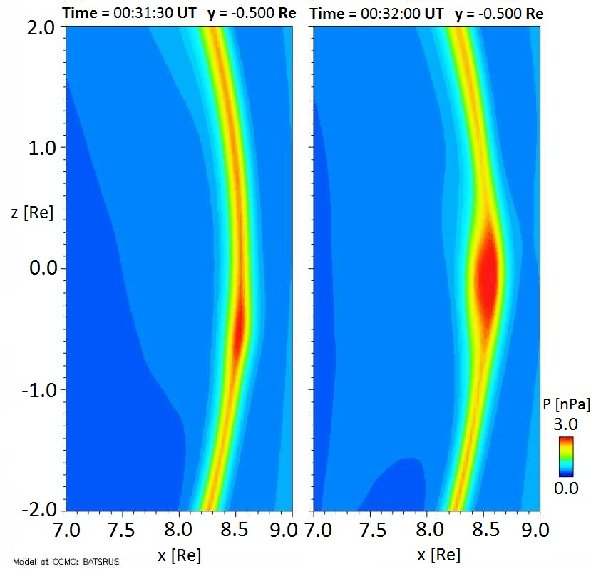
\includegraphics[scale=0.40]{pressaotempo1.jpg}
		\caption{Pressão de plasma no plano $x-z$ em $y= -0,5$ $Re$ no instante 00:31:30 (painel esquerdo) e 00:32:00 (painel direito). O Sol está situado à direita e a Terra à esquerda na origem do sistema.}
		\label{pressaotempo}
	\end{center}
\end{figure}


\begin{figure}
	\begin{center}
		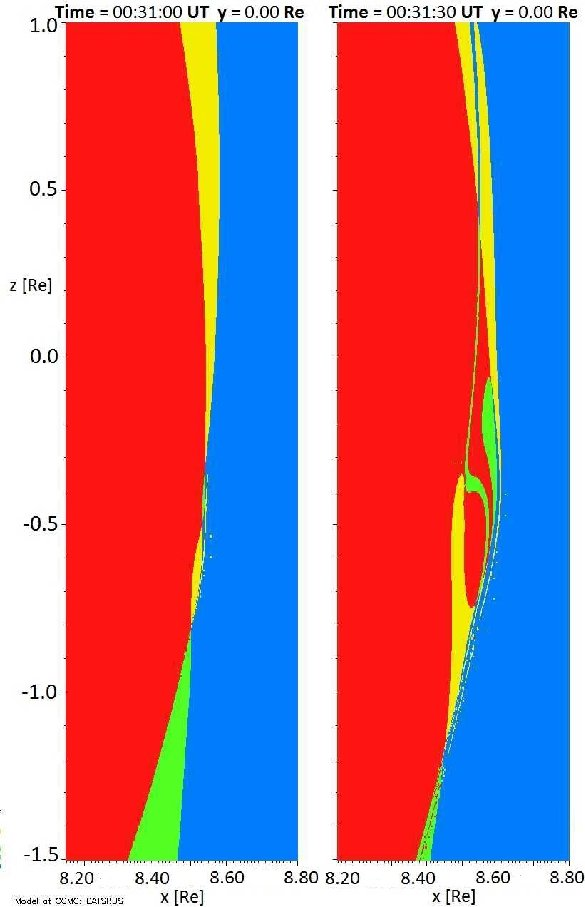
\includegraphics[scale=0.37]{topologia.jpg}
		\caption{Topologia magnética para os instantes de tempo 00:31:00 (painel esquerdo) e 00:31:30 (painel direito) no plano $x-z$ em $y= 0$. As regiões são identificadas em cores: vermelha corresponde à região em que as linhas estão conectadas à Terra, azul identifica as linhas ligadas ao Sol, verde corresponde às linhas que são conectadas ao sul da Terra e ao Sol, amarela para as linhas conectadas ao norte da Terra e ao Sol.}
		\label{topologia}
	\end{center}
\end{figure}

A análise da velocidade mostra que a direção de movimento do plasma é alterada pela reconexão magnética, como mencionado anteriormente. A Figura \ref{velocidade} mostra a velocidade do plasma no plano $x-z$ em $y= 0$ no tempo 00:31:30. A região vermelha indica que o plasma se propaga para o norte e a região azul corresponde ao plasma se movendo para o sul, resultante do processo de reconexão ocorrendo na magnetopausa. A estrutura se encontra entre $z= -1$ e $0$ $Re$ em 00:31:30 e se propagando para o norte como visto no parâmetro de topologia magnética da Figura \ref{topologia}. Entretanto, a velocidade do plasma na Figura \ref{velocidade} não evidencia a presença de tubos de fluxo magnético, mas somente uma região de reconexão em aproximadamente $z= -1$ $Re$, na interface entre as velocidades para o norte (vermelho) e o sul (azul). A velocidade do vento solar que contorna a magnetosfera ou do fluxo de plasma resultante da reconexão magnética, como nesse caso, pode ser mais alta que a velocidade da estrutura magnética, e assim, ocultar a visualização dos tubos de fluxo magnético. 

\begin{figure}
	\begin{center}
		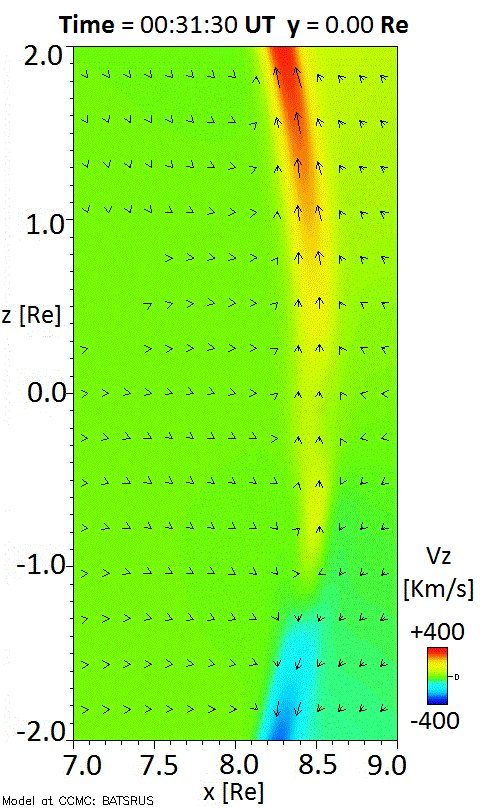
\includegraphics[scale=0.33]{velocidade.jpg}
		\caption{Velocidade do plasma no plano $x-z$ em $y= 0$ no tempo 00:31:30.}
		\label{velocidade}
	\end{center}
\end{figure}

Para se obter a apropriada identificação e a caracterização dos tubos, as variáveis pressão, topologia magnética e velocidade devem ser analisadas em conjunto, além de sua evolução espacial e temporal. Além disso, outras variáveis, como por exemplo, a densidade e a intensidade do campo magnético, podem ser investigadas de modo que a análise seja mais precisa e coerente. 


\section{Considerações finais}

Nesse trabalho foram apresentados os conceitos físicos envolvidos na formação de tubos de fluxo magnético na magnetosfera terrestre. A interação entre o vento solar, que arrasta o campo magnético interplanetário, e a magnetosfera está diretamente relacionada ao processo de reconexão magnética e à formação dos tubos de fluxo. 

Os FTEs, que foram primeiramente detectados por meio de dados observacionais em 1978, são formados por tubos de fluxo. Os modelos de Russell-Elphic, Lee-Fu, Southwood-Scholer e outros recentes são utilizados para descrever o tipo de reconexão que gera os FTEs e também a forma dos tubos que os compõem. 

Com o avanço da tecnologia e o aumento das missões espaciais na magnetosfera da Terra, muito tem se conhecido das características dos FTEs. O estudo da estrutura, da formação e da propagação de tubos de fluxo magnético em simulações, associados aos dados observacionais, demonstram um importante papel na busca da compreensão dos eventos FTEs. 


\section*{Agradecimentos}

P. P. Ferreira agradece o apoio do Conselho Nacional de Desenvolvimento Científico e Tecnológico (CNPq), processo No. 800010/2014-0. M. Silveira agradece ao apoio CNPq, processo No. 32906/2014-9. F.R. Cardoso agradece o apoio do CNPq, processo No. 454672/2014-4, e da
Fundação de Amparo à Pesquisa do Estado de São Paulo (FAPESP), processo No. 2015/21376-4. D. Koga agradece ao CNPq, processo No. 112886/2015-9. 


%\bibliographystyle{unsrt}
%\bibliography{referencias}

\begin{thebibliography}{10}
	
	\bibitem{gombosi2004}
	T.I. Gombosi, K.G. Powell, D.L.~De Zeeuw, C.R. Clauer, K.C. Hansen, W.B.
	Manchester, A.J. Ridley, I.I. Roussev, I.V. Sokolov, Q.F. Stout, et~al.
	\newblock {\em Computing in science \& engineering}, 6(2):14--35, 2004.
	
	\bibitem{russell2001}
	C.T. Russell.
	\newblock Solar wind and interplanetary magnetic field: A tutorial.
	\newblock In Howard J. Singer e George L.~Siscoe Paul~Song, editor, {\em Space
		Weather}, pages 73--89. American Geophysical Union, Washington DC, 2001.
	
	\bibitem{oliveira2016}
	D.M. Oliveira and M.V.D. Silveira.
	\newblock {\em Revista Brasileira de Ensino de F{\'\i}sica}, 38(1), 2016.
	
	\bibitem{nstc2015}
	National space weather strategy.
	\newblock Technical report, National Science and Technology Council, 2015.
	
	\bibitem{baumjohann1996}
	W.~Baumjohann and R.A. Treumann.
	\newblock {\em Basic space plasma physics}, volume~57.
	\newblock World Scientific, 1996.
	
	\bibitem{bittencourt}
	J.~A. Bittencourt.
	\newblock {\em Fundamentals of Plasma Physics}.
	\newblock José Augusto Bittencourt, 2003.
	
	\bibitem{costa2011}
	E.~Costa Jr., F.J.R.~Sim{\~o}es Jr., F.R. Cardoso, and M.V. Alves.
	\newblock {\em Revista Brasileira de Ensino de F{\'\i}sica}, 33(4):4301--4301,
	2011.
	
	\bibitem{kivelson1995}
	M.G. Kivelson and C.T. Russell.
	\newblock {\em Introduction to space physics}.
	\newblock Cambridge university press, 1995.
	
	\bibitem{sibeck2014}
	D.G. Sibeck and R.Q. Lin.
	\newblock {\em Journal of Geophysical Research: Space Physics},
	119(2):1028--1043, 2014.
	
	\bibitem{ezequiel2006}
	E.~Echer, M.V. Alves, and W.D. Gonzalez.
	\newblock {\em Revista Brasileira de Ensino de F{\i}sica}, 28(1):51--66, 2006.
	
	\bibitem{elphic1979}
	R.C. Elphic and C.T. Russell.
	\newblock In {\em Magnetospheric boundary layers}, volume 148, pages 43--50,
	1979.
	
	\bibitem{da2015}
	E.~Costa Jr. and M.V. Alves.
	\newblock {\em Revista Brasileira de Ensino de F{\'\i}sica}, 37(4), 2015.
	
	\bibitem{souza2016}
	V.M. Souza, M.V.D. Silveira, D.~Koga, and P.R. Jauer.
	\newblock {\em Revista Brasileira de Ensino de F{\'i}sica}, 38, 06 2016.
	
	\bibitem{lakhina1992}
	G.S. Lakhina.
	\newblock {\em Bulletin of the Astronomical Society of India}, 28:593--646,
	2000.
	
	\bibitem{treumann}
	R.~A. Treumann and W.~Baumjohann.
	\newblock {\em Advanced Space Plasma Physics}.
	\newblock Imperial College Press, London, 1997.
	
	\bibitem{zweibel2009}
	E.G. Zweibel and M.~Yamada.
	\newblock {\em Annual review of astronomy and astrophysics}, 47:291--332, 2009.
	
	\bibitem{gonzalez1974}
	W.D. Gonzalez and F.S. Mozer.
	\newblock {\em Journal of Geophysical Research}, 79(28):4186--4194, 1974.
	
	\bibitem{elphic1978}
	C.~T. Russell and R.~C. Elphic.
	\newblock {\em Space Science Reviews}, 22:681--715, 1978.
	
	\bibitem{southwood1988}
	D.J. Southwood, C.J. Farrugia, and M.A. Saunders.
	\newblock {\em Planetary and Space Science}, 36(5):503--508, 1988.
	
	\bibitem{scholer1988}
	M.~Scholer.
	\newblock {\em Geophysical research letters}, 15(4):291--294, 1988.
	
	\bibitem{lee1985}
	L.~C. Lee and Z.~F. Fu.
	\newblock {\em Geophysical Research Letters}, 12(2):105--108, February 1985.
	
	\bibitem{haerendel1978}
	G.~Haerendel, G.~Paschmann, N.~Sckopke, H.~Rosenbauer, and P.C. Hedgecock.
	\newblock {\em Journal of Geophysical Research}, 83:3195--3216, 1978.
	
	\bibitem{sonnerup1967}
	B.U. Sonnerup and L.J. Cahill.
	\newblock {\em Journal of Geophysical Research}, 72(1):171--183, 1967.
	
	\bibitem{siscoe1968}
	G.L. Siscoe, L.~Davis, P.J. Coleman, E.J. Smith, and D.E. Jones.
	\newblock {\em Journal of Geophysical Research}, 73(1):61--82, 1968.
	
	\bibitem{paschmann1982}
	G.~Paschmann, G.~Haerendel, I.~Papamastorakis, N.~Sckopke, S.J. Bame, J.T.
	Gosling, and C.T. Russell.
	\newblock {\em Journal of Geophysical Research}, 87(A4):2159--2168, April 1982.
	
	\bibitem{hesse1990}
	M.~Hesse, J.~Birn, and K.~Schindler.
	\newblock {\em Journal of Geophysical Research}, 95(A5):6549--6560, 1990.
	
	\bibitem{lee1993}
	L.C. Lee, Z.W. Ma, and A.~Otto.
	\newblock {\em Journal of Geophysical Research}, 98(A3):3943--3951, 1993.
	
	\bibitem{otto1995}
	A.~Otto.
	\newblock {\em Journal of Geophysical Research}, 100(A7):11,863--11,874, 1995.
	
	\bibitem{louarn2004}
	P.~Louarn, A.~Federov, E.~Budnik, G.~Fruit, J.~A. Sauvaud, C.~C. Harvey, and
	I.~Dandouras.
	\newblock {\em Geophysical Research Letters}, 31:L19805, 2004.
	
	\bibitem{cardoso2013}
	F.R. Cardoso, W.D. Gonzalez, D.G. Sibeck, M.~Kuznetsova, and D.~Koga.
	\newblock In {\em Annales Geophysicae}, volume~31, pages 1853--1866. Copernicus
	GmbH, 2013.
	
	\bibitem{Rijnbeeketal1982}
	R.P. Rijnbeek, S.W.H. Cowley, D.J. Southwood, and C.T. Russell.
	\newblock {}.
	\newblock {\em Nature}, 300:23--26, November 1982.
	
	\bibitem{BerchemandRussell1984}
	J.~Berchem and C.T. Russell.
	\newblock {}.
	\newblock {\em Journal of Geophysical Research}, 89(A8):6689--6703, August
	1984.
	
	\bibitem{Rijnbeeketal1984}
	R.P. Rijnbeek, S.W.H. Cowley, D.J. Southwood, and C.T. Russell.
	\newblock {}.
	\newblock {\em Journal of Geophysical Research}, 89(A2):786--800, February
	1984.
	
	\bibitem{Russelletal1996}
	C.T. Russell, G.~Le, and H.~Kuo.
	\newblock {}.
	\newblock {\em Advances in Space Research}, 18:197--205, 1996.
	
	\bibitem{SibeckandLin2010}
	D.G. Sibeck and R.Q. Lin.
	\newblock {}.
	\newblock {\em Journal of Geophysical Research}, 115:A04209, April 2010.
	
	\bibitem{Russelletal1985}
	C.T. Russell, J.~Berchem, and J.G. Luhmann.
	\newblock {}.
	\newblock {\em Advances in Space Research}, 5:363--368, 1985.
	
	\bibitem{Fearetal2009}
	R.C. Fear, S.E. Milan, A.N. Fazakerley, and K.H. Forna{\c c}on.
	
	\bibitem{Silveira2015}
	M.V.D. Silveira.
	\newblock {\em Study of flux transfer events observed at the Earth's
		magnetopause by THEMIS satellites}.
	\newblock PhD thesis, Instituto Nacional de Pesquisas Espaciais (INPE), S{\~a}o
	Jos{\'e} dos Campos, 2015-03-03 2015.
	
	\bibitem{Elphic1995}
	R.~C. Elphic.
	\newblock volume~90, pages 225--233.
	\newblock American Geophysical Union, 1995.
	
	\bibitem{Paschmannetal1982}
	G.~Paschmann, G.~Haerendel, I.~Papamastorakis, N.~Sckopke, S.~J. Bame, J.~T.
	Gosling, and C.~T. Russell.
	\newblock {}.
	\newblock {\em Journal of Geophysical Research}, 87(A4):2159--2168, April 1982.
	
	\bibitem{Owenetal2001}
	C.J. Owen, A.~Marchaudon, M.W. Dunlop, A.N. Fazakerley, J.M. Bosqued, J.P.
	Dewhurst, R.C. Fear, S.A. Fuselier, A.~Balogh, and H.~Reme.
	\newblock {\em Journal of Geophysical Research}, 113(A7):n/a--n/a, 2008.
	\newblock A07S04.
	
	\bibitem{Fearetal2008}
	R.C. Fear, S.E. Milan, A.N. Fazakerley, E.A. Lucek, S.W.H. Cowley, and
	I.~Dandouras.
	\newblock {}.
	\newblock {\em Annales Geophysicae}, 26(8):2353--2369, August 2008.
	
	\bibitem{kelley}
	Michael Kelley.
	\newblock {\em The Earth's Ionosphere- Plasma physics and Electrodynamics}.
	\newblock Academic Press, 2009.
	
	\bibitem{pinnock03}
	M.~Pinnock, G.~Chisham, I.~J. Coleman, M.~P. Freeman, M.~Hairston, and
	J.P.Villain.
	\newblock The location and rate of dayside reconnection during an interval of
	southward interplanetary magnetic field.
	\newblock {\em Annales Geophysicae}, 21:1467--1482, Jul. 2003.
	
	\bibitem{gary90}
	R.~C. Elphic and S.~P. Gary.
	\newblock Isee observations of low frequency waves and ion distribution
	function evolution in the plasma sheet boundary layer.
	\newblock {\em Geophysical Research Letters}, 17:2023--2026, 1990.
	
	\bibitem{Elphicetal1990}
	R.C. Elphic, M.~Lockwood, S.W.H. Cowley, and P.E. Sandholt.
	\newblock {}.
	\newblock {\em Geophysical Research Letters}, 17:2241--2244, November 1990.
	
	\bibitem{GlassmeierandStellMacher1996}
	K.H. Glassmeier and M.~Stellmacher.
	\newblock {}.
	\newblock {\em Advances in Space Research}, 18:151--160, 1996.
	
	\bibitem{Neudeggetal2000}
	D.A. Neudegg, S.W.H. Cowley, S.E. Milan, T.K. Yeoman, M.~Lester, G.~Provan,
	G.~Haerendel, W.~Baumjohann, B.~Nikutowski, J.~B{\"u}chner, U.~Auster, K.H.
	Fornacon, and E.~Georgescu.
	\newblock {}.
	\newblock {\em Annales Geophysicae}, 18:416--435, April 2000.
	
	\bibitem{toth05}
	G.~Toth and et~al.
	\newblock Space weather modeling framework: a new tool for the space science
	community.
	\newblock {\em Journal of Geophysical Research}, 110:A12226, 2005.
	
	\bibitem{powell99}
	K.G. Powell, P.L. Roe, T.J. Linde, T.I. Gombosi, and D.L.~De Zeeuw.
	\newblock A solution adaptative upwind scheme for ideal magnetohydrodynamics.
	\newblock {\em Journal of Computational Physics}, 154:284--309, 1999.
	
	\bibitem{dorelli09}
	J.~C. Dorelli and A.~Bhattacharjee.
	\newblock On the generation and topology of flux transfer events.
	\newblock {\em Journal of Geophysical Research}, 114:A06213, 2009.
	
	\bibitem{raeder06}
	J.~Raeder.
	\newblock Flx transfer events: 1.generation mechanism for strong southward imf.
	\newblock {\em Annales Geophysicae}, 24:381--392, 2006.
	
\end{thebibliography}
